\documentclass{article}
\usepackage{graphicx}
\usepackage[dvipsnames]{xcolor}
\usepackage{xspace}  % trailing spaces after \newcommands. 

\begin{document}

\newcommand{\hl}[1]{\textcolor{red}{#1}}
% \newcommand{\nutstore}{\texttt{NutrientStore\xspace}}
% \newcommand{\nutstores}{\texttt{NutrientStores\xspace}}
\newcommand{\nutstore}{\texttt{NutrientStore }}
\newcommand{\nutstores}{\texttt{NutrientStores }}

\title{GutSim Design and Reasoning}
\author{Mark N. Read}

\maketitle

This document is intended to accompany the paper \hl{INSERT PAPER TITLE HERE}. 

%%%%%%%%%%%%%%%%%%%%%%%
\section{Agent based modelling}

GutSim is an agent based model. 
Each individual microbe within the gut is explicitly represented as an individual entity with its own bespoke state, housed within a spatially explicit environment with a local profile of substrate. 
Its state dictates a microbe's fate, and its behaviour within the environment. 
The sections that follow describe the modelling of diet, relevant host digestive and physiological processes, and the behaviours of individual microbes. 

%%%%%%%%%%%%%%%%%%%%%%%
\section{Modelling dietary intake}

GutSim was designed around the diets utilised in a comprehensive investigation of how dietary macronutrient distribution and energy density impacts many aspects of host physiology \cite{Solon-Biet2014}. 

The study defined ten macronutrient ratios (protein:carbohydrate:fat \%). 
A total of thirty diets were constructed around these macronutrient distributions by diluting the ten base diets with cellulose to achieve three energy densities: 2, 3 and 4 kcal/gram of chow. 
Cellulose is nutritionally inaccessible to both mouse and microbe, and thus mice consume less accessible energy per gram of chow on the low energy densities. 
Only 25 of these 30 diets were advanced in the study as the remaining five are nutritionally non-viable for mice. 
The study involved nearly 900 mice housed across 250 cages. 
The daily intakes of each cage was recorded, and thus the average daily mouse intake for each cage calculated. 
The dietary intakes of these 250 cages have been implemented within GutSim. 

The diets comprised a single dietary protein, casein. 
Three (non-cellulose) carbohydrates were included: sucrose, wheat starch and dextrinized cornstarch. 
Dextrinization is a process involving heating up starch to create disaccharides. 
Wheatstarch is more digestion resistant than dextrinised cornstarch. 
The dietary fat was soyabean oil. 
Beyond its dilution of other dietary macronutrients, GutSim does not incorporate any notion of dietary fat; at time of writing, we judge insufficient to be known of its interaction with the microbiome to accurately model it.
Cellulose is accounted for within the model, as it serves as a bulking agent within a modelled gut of limited capacity and thus impacts defecation dynamics.  

Mice are more active during the dark phase than the light phase, and this includes their dietary intakes.
We simulate 2/3rds of daily dietary intake to be consumed during the dark phase, and the remainder during the light phase; constant intake rates are assumed within each phase.

%%%%%%%%%%%%%%%%%%%%%%%
\section{Host sequestration of dietary nutrients}

We assume that the host absorbs all dietary sucrose, and hence it is inaccessible to the modelled microbiome. 
For wheatstarch, dextrinised cornstarch and protein components of diet, we assume a saturating capacity for the host to sequester these macronutrients in the small intestine. 
The proportion of ingested macronutrient sequestered by the host reduces as the quantity ingested increases:

\begin{center}
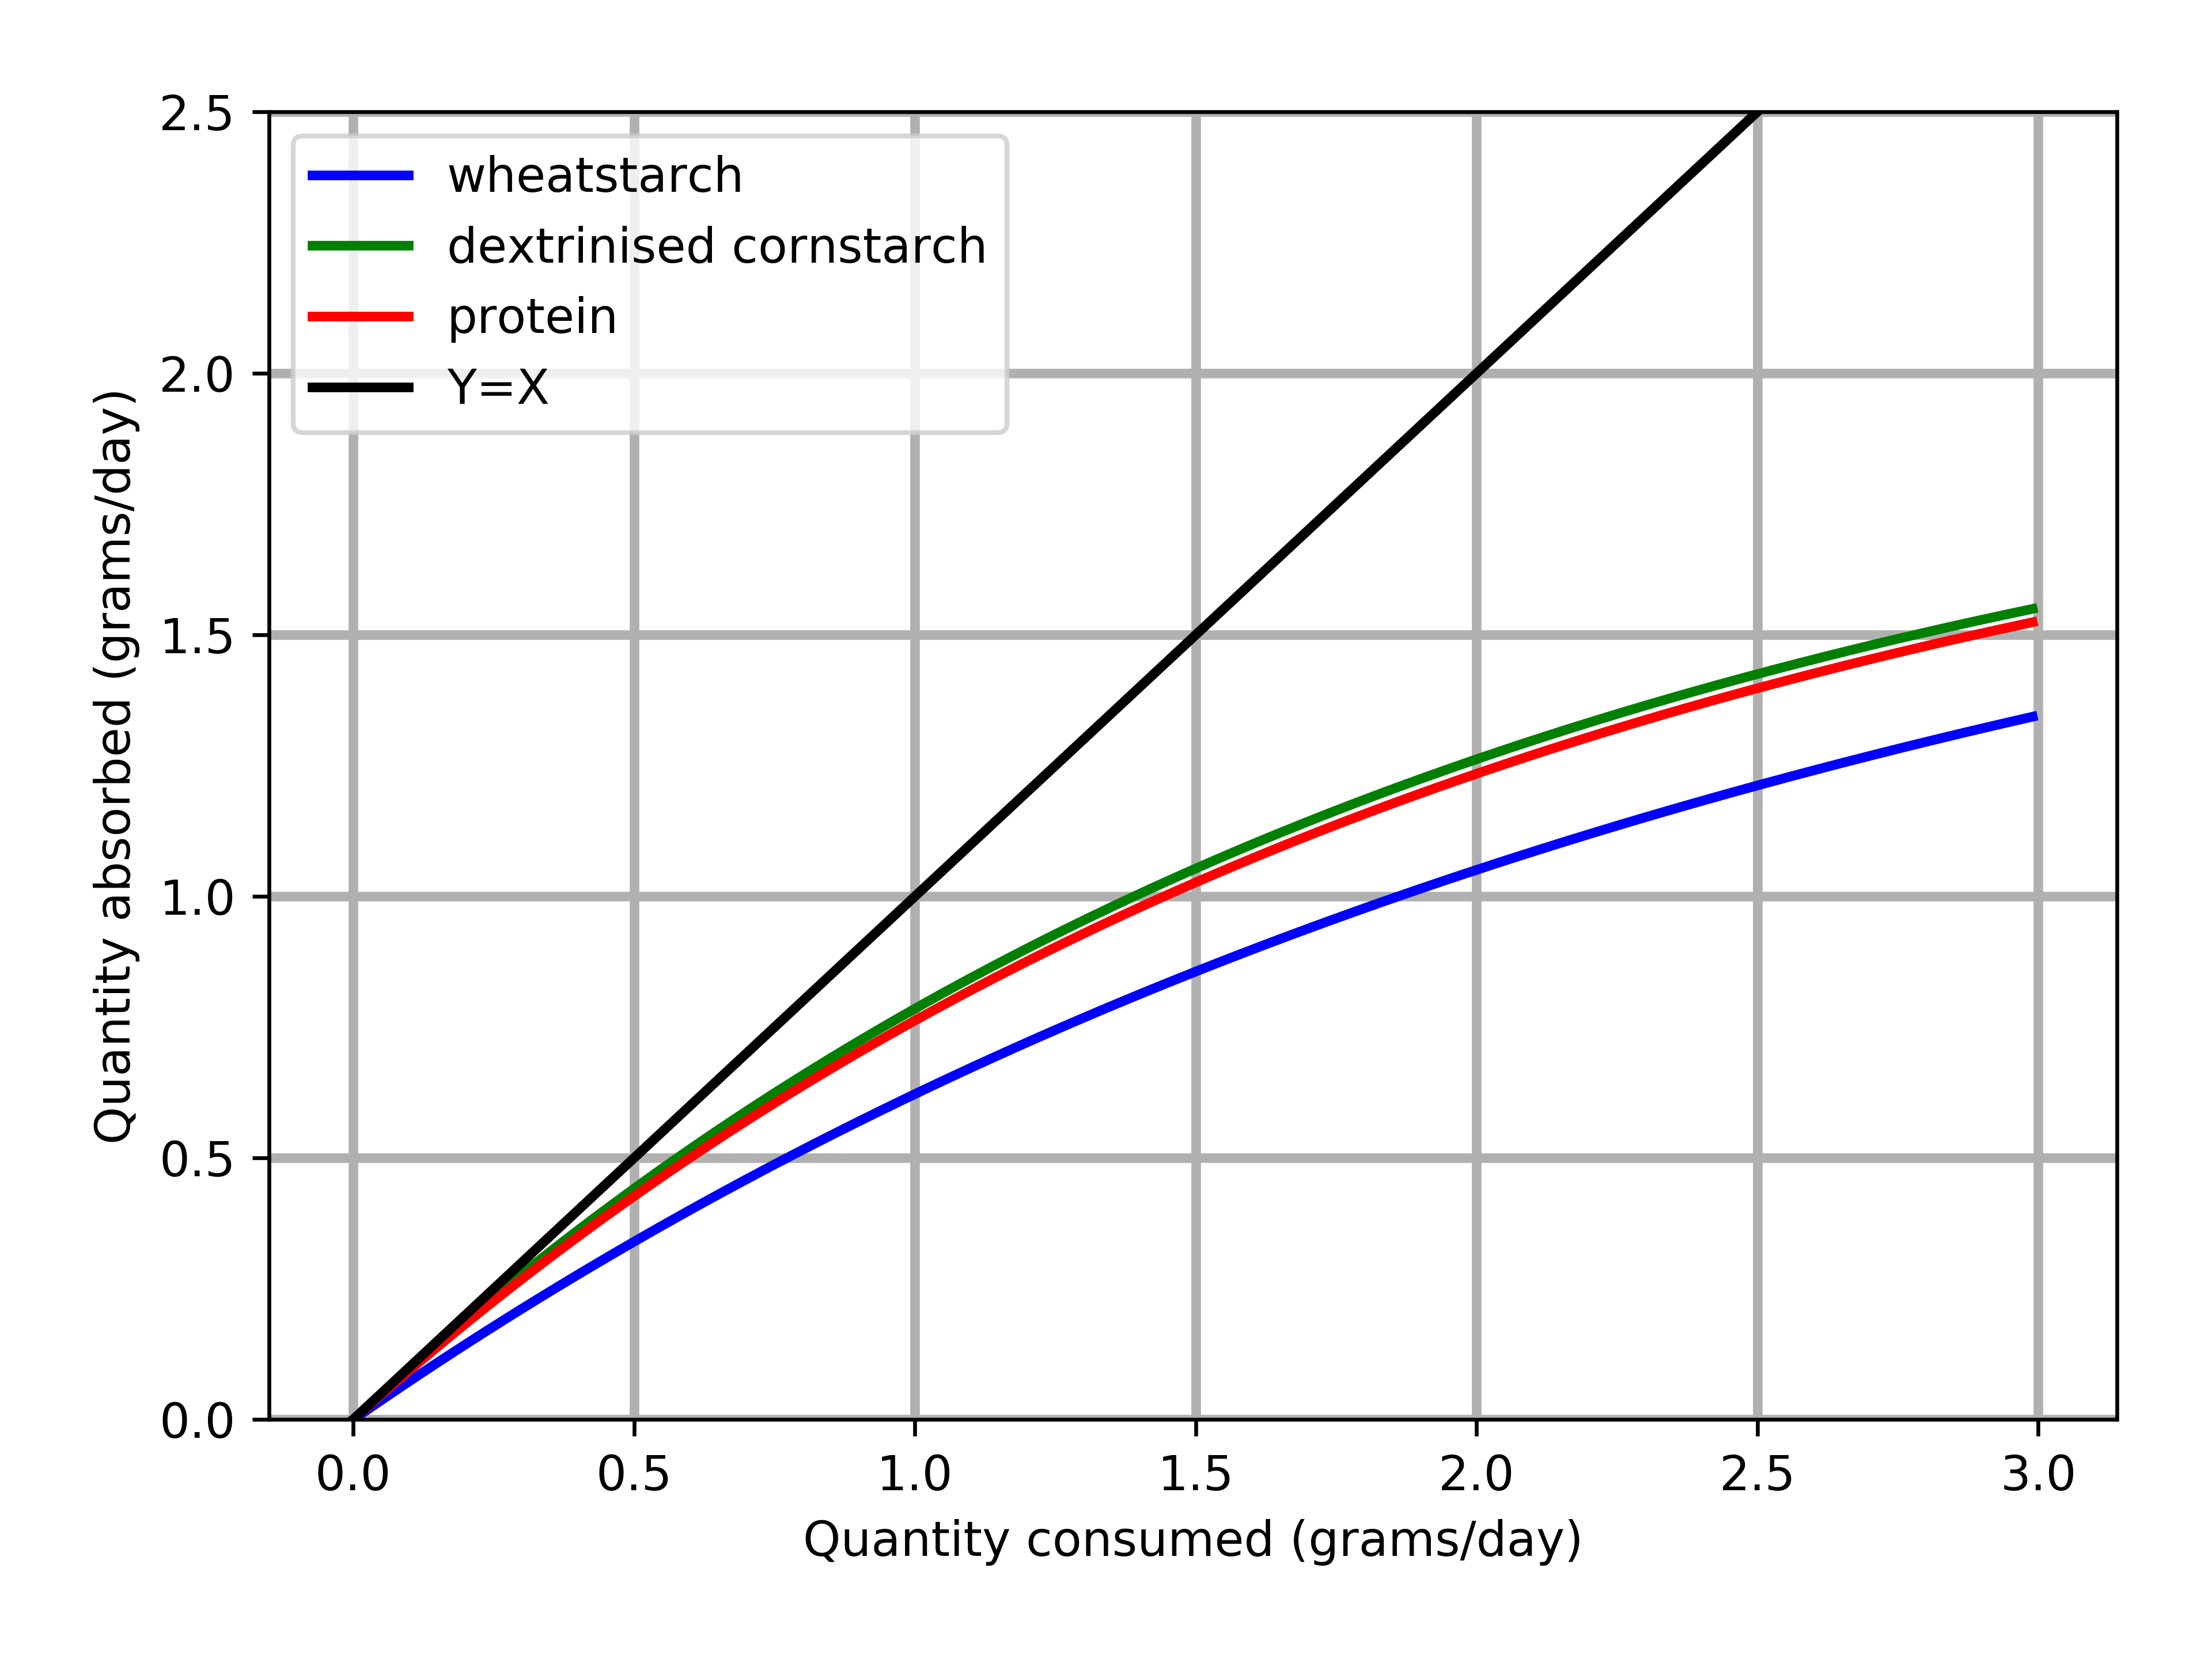
\includegraphics[width=12cm]{../probability-curves/si_absorbed.png}
\end{center}

We model this relationship, quantity of ingested dietary component ($x$) that the host sequesters ($y$), using the following equation:

\begin{equation}
  y = c (1 - e^{-kx})  
\end{equation}

We assume that the absolute maximum quantity of each dietary component that the mouse can sequester through the small intestine is 2g/day (this was arbitrarily selected). 
Hence, the functions approach this asymptote as intake increases.
Accordingly, we set c = 2.  

Our calibration of the slope of this line is based on data from ileostomy recipients~\cite{Silvester1995,Isaksson1983,Silvester1995a,Englyst1986,Englyst1985}. 
These patients have parts parts of their gastrointestinal tract removed, and the ileum is diverted to a artificial opening in the abdominal wall. 
Dietary studies conducted on ileostomates can ascertain the dynamics of host sequestration of dietary intake by the small intestine. 
Note that a confounding factor is typically how endogenous sources of nitrogen and carbon have been accounted for.
Further, the recovery of dietary components in effluent is highly sensitive to the type of e.g. carbohydrate, and its culinary preparation. 
The carbohydrates used in these mouse diets were not cooked, rendering them relatively digestion resistant. 
Based on the aforementioned studies, we assume that a `standard' quantity of intake of each dietary component will result in a percentage of said component reaching the large intestines as given below.
The most `standard' of the mouse diets was the 14-57-29 (P:C:F \%) at 4kcal/g. This equates the the following absolute quantities of each diet component being consumed
\begin{description}
  \item[Protein:] 12\% of 0.37g daily intake reaches the large intestine
  \item[Wheatstarch:] 30\% of 0.34g daily intake reaches the large intestine
  \item[Dextrinised cornstarch:] 6\% of 0.24g daily intake reaches the large intestine
\end{description} 

With quantity ingested and sequestered by the host known, the following rearrangement of the above equation is be used to calculate $k$ for each dietary component. 

\begin{equation}
  k = -ln(1 - (x * y) / 2) / x
\end{equation}

% Another consideration in these calibrations is that the quantity of dietary component sequestered by the host cannot exceed what was ingested; this was verified. 

%%%%%%%%%%%%%%%%%%%%%%%
\section{The modelled gut environment}

We model microbes as inhabiting a 1-dimensional space, longitudinally representing the mouse cecum and large intestine. 
The 1-dimensional gut contains a sequence of discretised, well-mixed spatial compartments (named \nutstore in GutSim).
Each NutrientStore maintains a local quantity of microbial substrate, metabolically inert waste, and biomass. 
GutSim adheres to conservation of mass between dietary input, fecal mass, and gut contents. 
Simulated time is discretised into 6min chunks, at which points all states within the model are updated. 
Accordingly, dietary components (post-host sequestration) representing 6min of consumption are input as a \nutstore to proximal modelled gut.

Individual microbes are stored as a sequence that is mapped onto the NutrientStores; numerous microbes will be mapped onto each \nutstore.
The combined cecal and colon contents of the mouse weigh around 2.25g, which we assume to be 70\% water; hence 0.675g of dry weight. 
We assume a mouse voids 10\% of its cecal and colon contents per hour during the dark phase, and half this during the light phase. 
The defecation rate is quintupled if modelled gut contents exceeds 0.675g. 
A cumulative count of mass to be defecated is maintained, updated every 6min, and when this exceeds the mass contained in the most distal \nutstore, that \nutstore and any associated microbes are removed and the mass count adjusted accordingly. 

The number of \nutstores the modelled gut contains is variable, the result of modulated intake rates.
A greater number of \nutstores that contain less mass can be accommodated in the gut. 
This manifests in some graphs (e.g. spatiotemporal heatmaps of microbial dynamics or substrate availability within the modelled gut) depicting a seemingly variable length of gut; this is not the case, the gut is modelled as being a constant 8cm in length. 

GutSim represents peristalsis such that the order of individual microbes within the sequence in which they are housed is locally shuffled. 
This is necessary to prevent those microbes most proximal in the sequence gaining repeated preferential access to dietary nutrient as it is input into the gut and experiencing a growth advantage that results in washout of all other microbe types. 
Modelled peristalsis also entails some mixing of substrates across neighbouring \nutstores. 
In both cases, the degree of spatial rearrangement is modelled through a gaussian distribution such short translational movements are most likely.
The gaussian-based shuffling is applied iteratively over the entire length of the modelled gut, repeated at each time increment. 


%======================
\subsection{Host provision of mucin}

GutSim models host excretion of mucin into the gastrointestinal tract. 
Mucin is secreted at a constant rate (not modulated by light/dark phase, or diet) uniformly along the length of the modelled gut. 
This is implemented as supplementing each \nutstore in the modelled gut with the protein and glycan components of mucin at each time increment. 
The quantities secreted were calculated as follows. 
Host intestinal tissues generate a mucin layer of 82 micron depth per hour \cite{Ermund2013} over a lower intestinal area of area 11.8cm$^2$ \cite{Wolczuk2011}.
We assume 1cm3 of this mucin layer to weigh 1g.
Water comprises 90\% of this layer \cite{Macfarlane2005}, and of the remaining glycoprotein component 80\% is estimated to constitute glycans versus protein \cite{Bansil2006}. 

%%%%%%%%%%%%%%%%%%%%%%%
\section{Modelling microbe cells}

We assume carbon (C) and nitrogen (N) to be the nutrients most readily limiting microbial growth in the gut ecosystem; all other nutrients are assumed to be available in non-limiting quantities. 
A microbe's fate is determined by its access to C and N, which it requires in a ratio of 5.2C:1N, representing the weight of C and N within microbes undergoing the exponential growth phase: \cite{Vrede2002,Chrzanowski1996}.

Microbial metabolism entails the sequestration of nutrients from the environment, excluding their use by other microbes. 
This has been abstracted as microbes `internalising' the C and N components of macronutrients in their corresponding \nutstore; the corresponding macronutrient quantities are removed from the local environment.
This `internalisation' occurs at constant rate. 
Microbes are confined to accessing only select macronutrients as per their guild membership, as described in section~\ref{sec:guilds}.

`Internalised' C and N is assumed to be metabolically engaged, and as such the quantities of each in these internalised stores subject to standard exponential decay with time. 
This represents C and N being converted into metabolically inert compounds. 
We assume this rate to be four-fold higher for C than for N:
\begin{equation}
dM / dt = M / L
\end{equation}
Where $M$ represents either internalised C or N, and half-life $L$ is 10 hours for N and 2.5 hours for C.

Given 5.2:1 C:N ratio, the \emph{limiting resource level} ($R$) of the cell can be calculated; excess of either internalised C and N beyond this ratio confers no behavioural change. 
An individual microbe's probabilities of death and division in an hour are based on its limiting resource level thus:
\begin{center}
  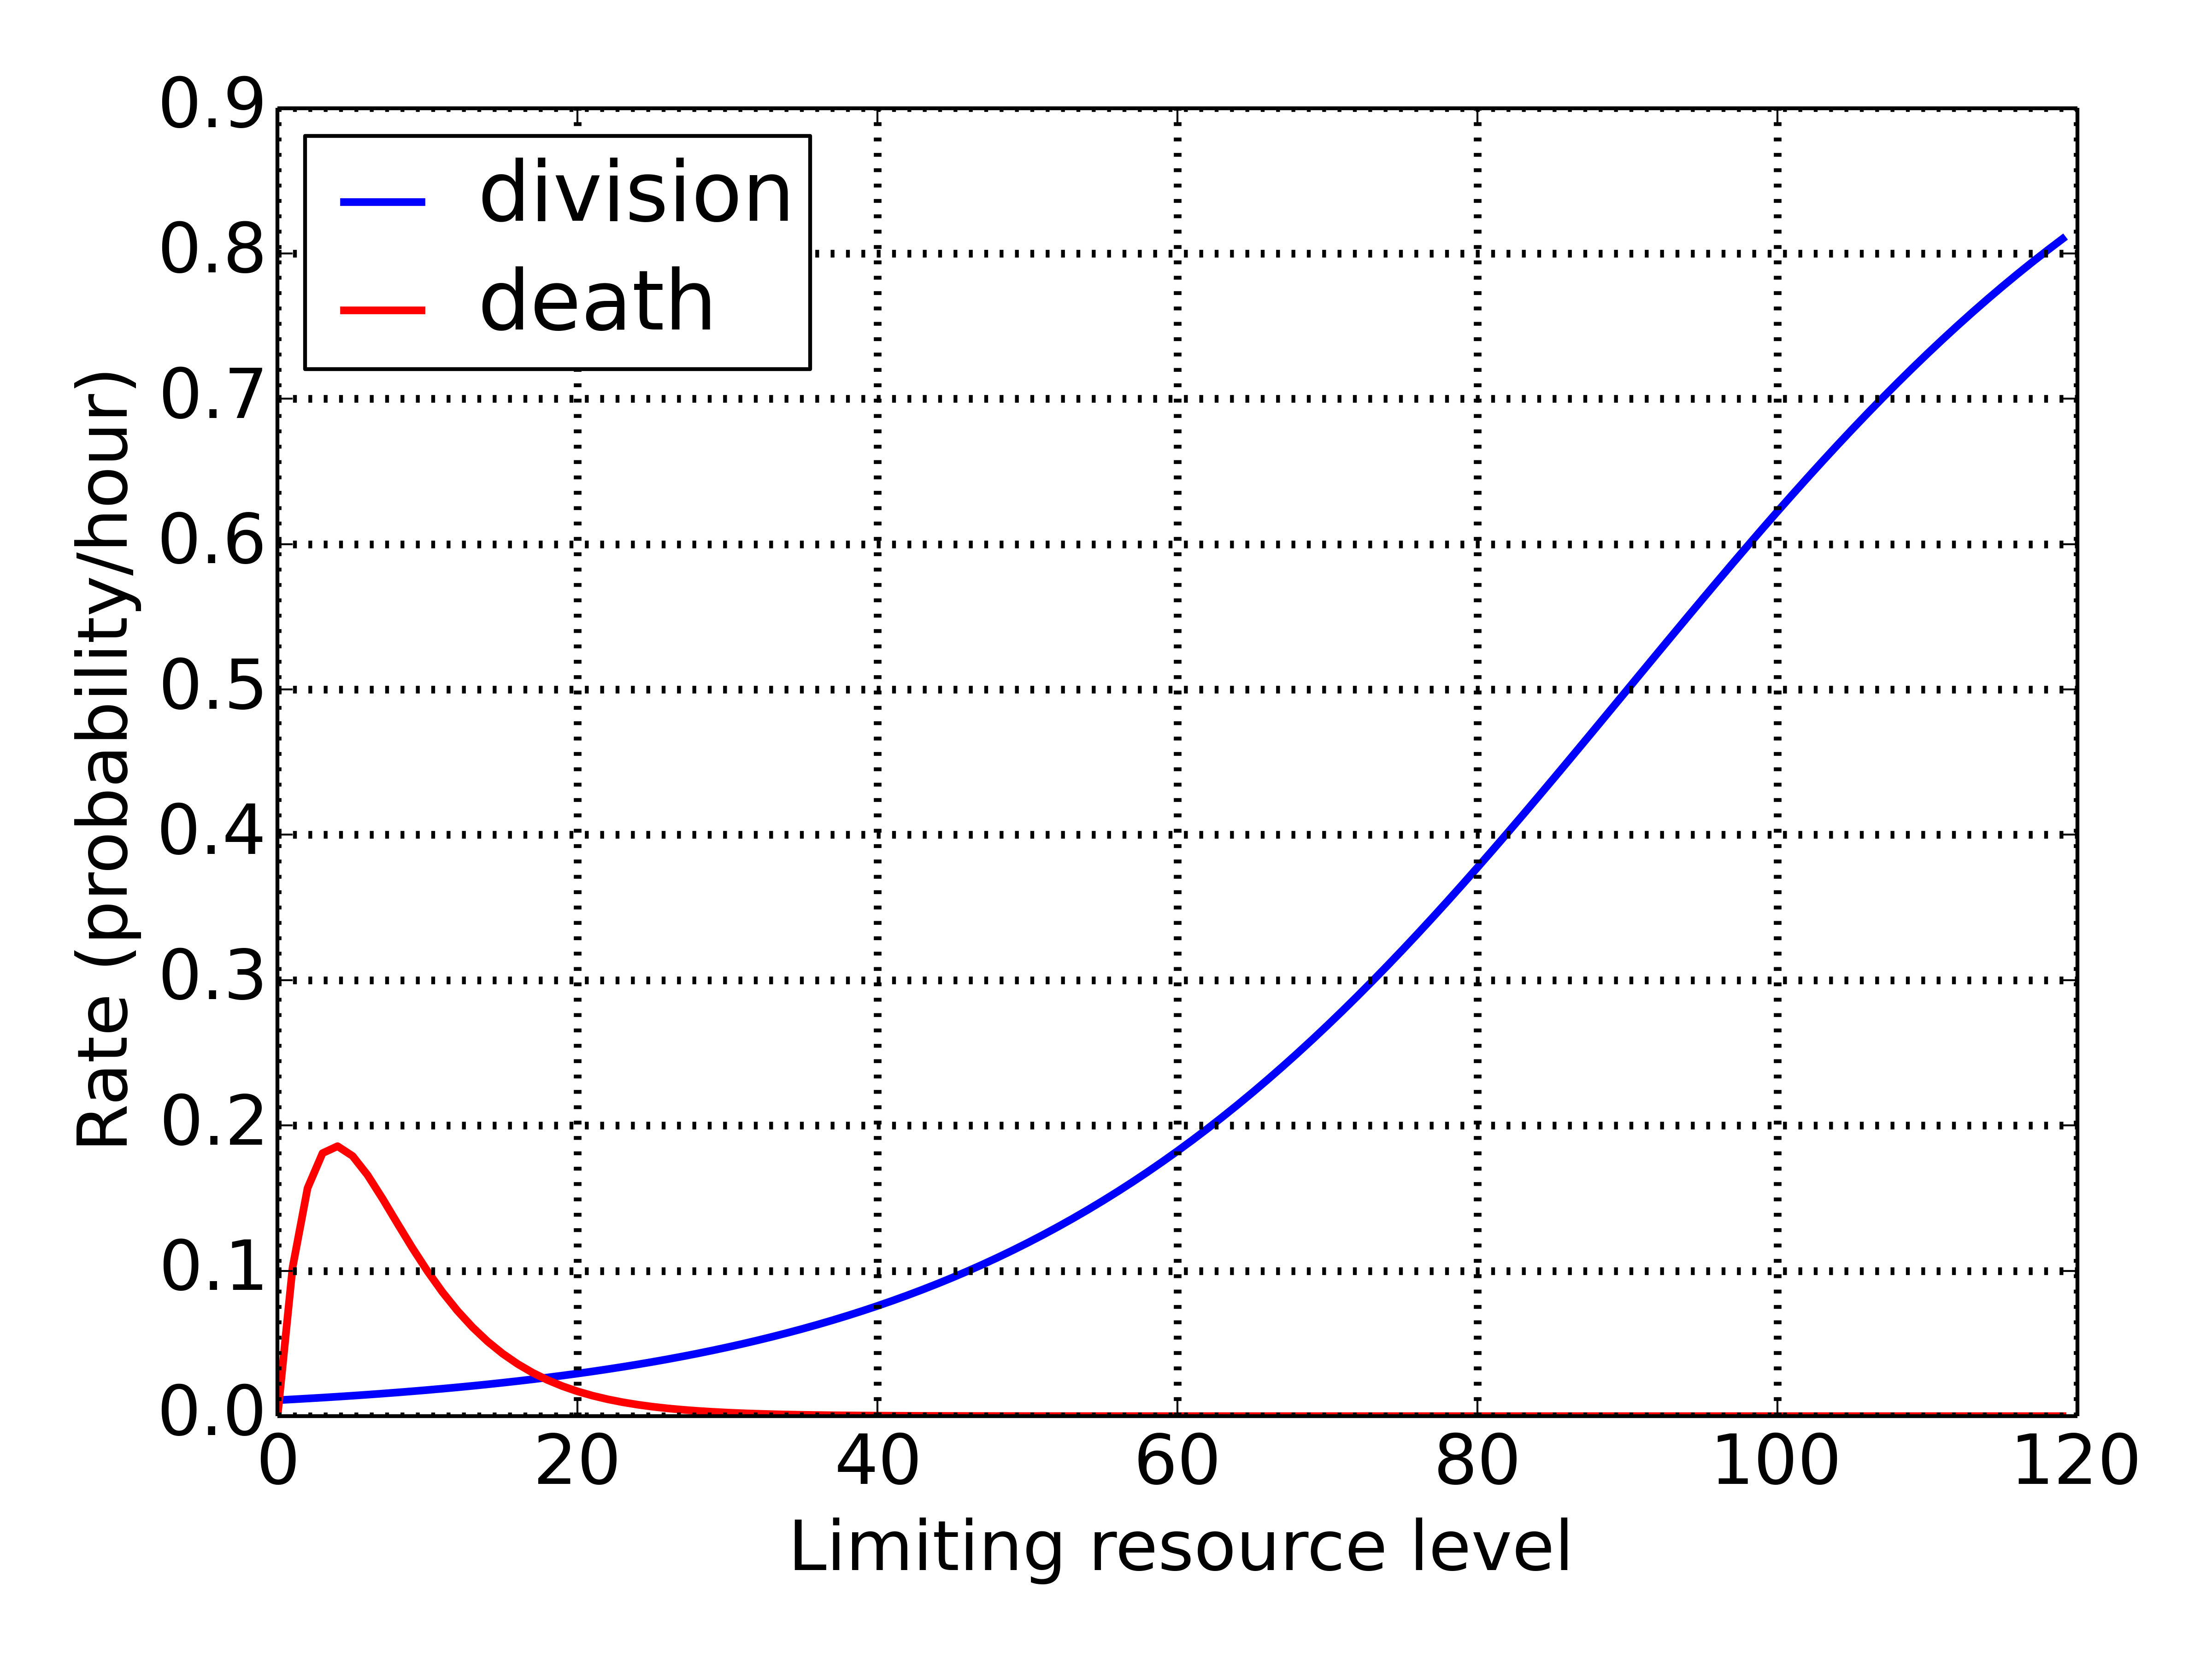
\includegraphics[width=10cm]{../probability-curves/death_growth_rates.png}
\end{center}
\begin{equation}
  P(division) = \frac{1}{(1 + e ^{ -0.05 \cdot (R - 90)})} \cdot tau
\end{equation}
\begin{equation}
  P(death) = e^{-R / 5} - e^{-R / 3} \cdot tau
\end{equation}

These equations are evaluated, for each individual microbe, at every time increment ($\tau$).
These probabilities, which can be queried for every modelled microbe at every point in time, allow articulation of population growth and death rates 
Microbial substrate uptake is modulated by which nutrient, C or N, is limiting; within a small tolerance, microbes will not uptake substrates devoid of limiting nutrients. 
Microbes are modelled as being weightless, and any substrate mass that they internalise is immediately reflected in corresponding mass of metabolically inert material in the microbe's corresponding \nutstore.
Of this metabolically inert mass, 30\% is removed, representing absorption of microbial metabolites by the host, and the remaining 70\% resides in the modelled gut. 
this ensures a conservation of mass input and output of the gut.


%======================
\subsection{Guilds capture strategies for C and N acquisition.}
\label{sec:guilds}

Guilds are confined to utilisation of a single carbohydrate and a single protein substrate.
The carbohydrate source contributes only carbon (C) to the microbe, and carbohydrates are modelled to constitute 44\% C by weight \cite{Rouwenhorst1991}. 
Protein contributes both C and nitrogen (N) to a microbe, and constitutes 53\% and 16\% of both by weight respectively \cite{Rouwenhorst1991}.
Of substrate mass that is internalised, C and N contents are added to the microbe's internal stores. 
We define six guilds around the dietary components of a mouse dietary intervention study that GutSim is aligned with. 
The two protein sources dietary protein (casein) and the protein component of mucin. 
The three carbohydrate sources are dietary wheatstarch, dextrinised cornstarch and the glycan component of mucin. 
The intersection of these components yields the six guilds. 

%%%%%%%%%%%%%%%%%%%%%%%
\section{Model initialisation}

The model commences with each of the six guilds represented by 100 microbes, shuffled along the length of the gut. 
The modelled gut is populated with \nutstores representing 24h of dietary intake prior to commencement of model execution. 
A small number of microbes representing each guild are input to the model each day, representing migration of microbes from further up the gastrointestinal tract and from the environment (diet). 


\section{References}
\bibliographystyle{plain}
\bibliography{references}

\end{document}